%% Default Latex document template
%%
%%  blake@rcs.ee.washington.edu

\documentclass[letterpaper]{article}

% Uncomment for bibliog.
%\bibliographystyle{unsrt}

\usepackage{graphicx}
\usepackage{lineno}
\usepackage{amsmath}
%\usepackage{fancyhdr}

%%%%%%%%%%%%%%%%%%%%%%%%%%%%%%%%%%%%%%%%5
%
%  Set Up Margins
\input{templates/pagedim.tex}

%
%        Font selection
%
%\renewcommand{\rmdefault}{ptm}             % Times
%\renewcommand{\rmdefault}{phv}             % Helvetica
%\renewcommand{\rmdefault}{pcr}             % Courier
%\renewcommand{\rmdefault}{pbk}             % Bookman
%\renewcommand{\rmdefault}{pag}             % Avant Garde
%\renewcommand{\rmdefault}{ppl}             % Palatino
%\renewcommand{\rmdefault}{pch}             % Charter


%%%%%%%%%%%%%%%%%%%%%%%%%%%%%%%%%%%%%%%%%%%%%%%%%
%
%         Page format Mods HERE
%
%Mod's to page size for this document
\addtolength\textwidth{0cm}
\addtolength\oddsidemargin{0cm}
\addtolength\headsep{0cm}
\addtolength\textheight{0cm}
%\linespread{0.894}   % 0.894 = 6 lines per inch, 1 = "single",  1.6 = "double"

% header options for fancyhdr

%\pagestyle{fancy}
%\lhead{LEFT HEADER}
%\chead{CENTER HEADER}
%\rhead{RIGHT HEADER}
%\lfoot{Hannaford, U. of Washington}
%\rfoot{\today}
%\cfoot{\thepage}



% Make table rows deeper
%\renewcommand\arraystretch{2.0}% Vertical Row size, 1.0 is for standard spacing)

\begin{document}
\section*{Path Optimization: Brute Force Search}

\section{Basics}

\subsection{Notation}
The goal is to search a grid of points in the  space consisting of points  $P_i = \{X_i, V_i\} = \{x,y,z,\dot{x},\dot{y},\dot{z}\}$ within bounds:
\[
-1 < x < 1, \;
-1 < y < 1, \;
-1 < z < 1, \;
-1 < \dot{x} < 1, \;
-1 < \dot{y} < 1, \;
-1 < \dot{z} < 1, \;
\]


We wish to visit all the points with as low a cost as possible.
We will set up a grid with $N$ points per axis, for a total of $6^N$ points.

A {\it trajectory}, $T_{ij}$ between two points in this space, $T(P_i,P_j)$, is a route through
the space from $P_i$ to $P_{i+1}$ with the properties

\beq \label{firstconstraint}
\Delta X (T_{ij}) = \frac{X_{i+1}-X_i}{\Delta t}
\eeq
%
% \beq
% | \frac {\Delta V} {\Delta t} |_\infty  < a_{max}
% \eeq
% \beq
% | \frac {\Delta V} {\Delta t} |_\infty < v_{max}
% \eeq
% \beq \label{complexconstraint}
% |\Delta V +  \frac {\Delta X}{\Delta t} |_\infty < v_{max}
% \eeq

% Figure 1
\begin{figure}\centering
%   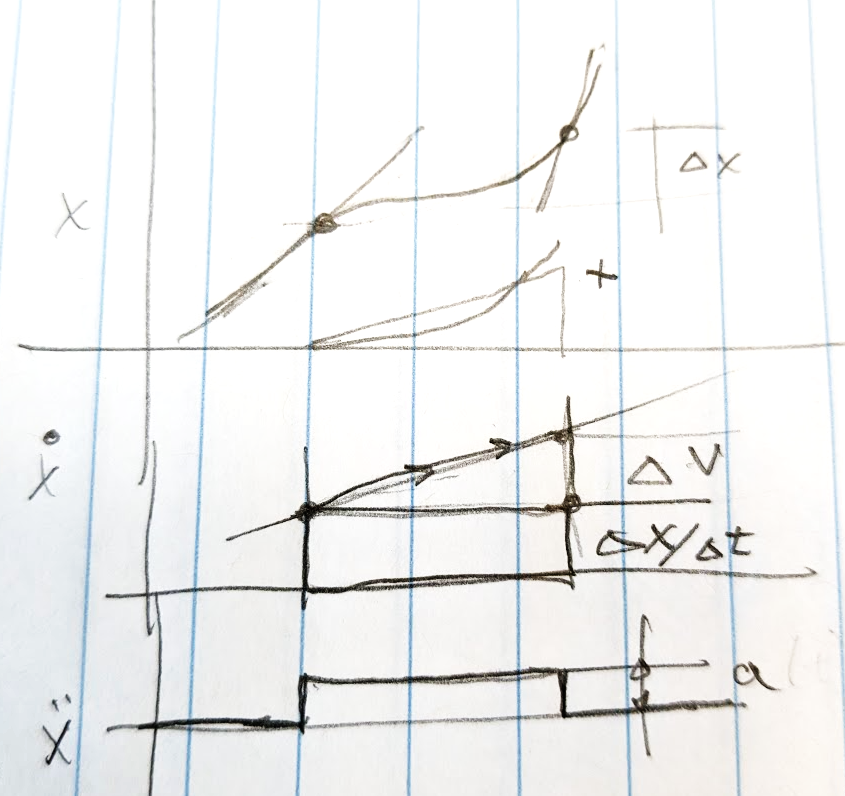
\includegraphics[width=3.0in]{basicTraj.png}
  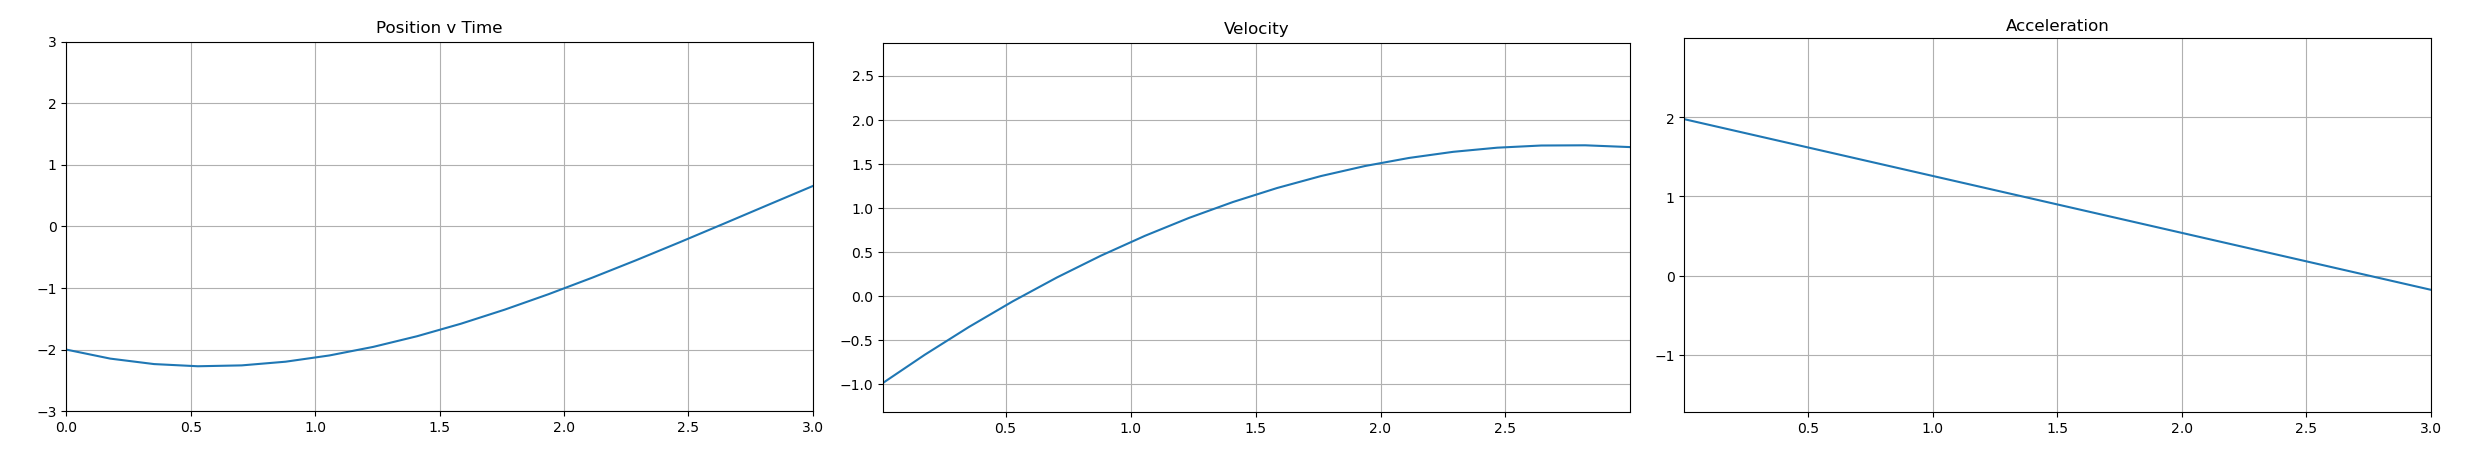
\includegraphics[width=\textwidth]{computedTraj.png}
  \caption{}\label{basicTraj}
\end{figure}

% Constraint eqn (\ref{complexconstraint}) can be seen from Figure \ref{basicTraj}.
%
% Two components of ${V}_i$
% are shown, one arising from $\Delta X$ and another arising from $\Delta V$.


\subsection{Trajectories between points}

A {\bf Trajectory}, $T_{ij}$ connects point $P_i$ to point $P_j$
in phase space with a time function $x(t), 0<t<\Delta t $.  To meet the constraints
\beq \label{trajConstraints}
x(0) = X_i, \; x(\Delta t) = X_j, \; \dot{x}(0) = V_i, \;
\dot{x}(\Delta t) = V_j
\eeq
we can use a 3rd order polynomial having four unknown constants:
\beq
\begin{aligned} \label{polyTraj}
x(t) & = a_0 + a_1t + a_2t^2 + a_3t^3 \\
v(t) & = \hspace{7mm}  a_1+2a_2t + 3a_3t^2 \\
a(t) & = \hspace{16mm}  2a_2 + 6a_3 t \\
\end{aligned}
\eeq

A typical trajectory of this type, computed for
\beq
x(0) =  -2, \; v(0) = -1, \qquad  x(\Delta t) = 1.5, \; v(\Delta t) = 1.5
\eeq
is given in Figure \ref{basicTraj}.

The constants are solved as follows:
\beq
a_0 = x(0),  a_1 = v(0)
\eeq
defining some intermediate terms:

\beq
\Delta x = x(\Delta t)-x(0) \qquad \Delta v = v(DT)-v(0)
\eeq

\beq
b0 = \Delta t \qquad b1 = {\Delta t}^2 \qquad b2 = {\Delta t}^3
\eeq

\beq
b3 = 2\Delta t \qquad b4 = 3{\Delta t}^2
\eeq
then
\beq
a_3 = \frac {b1 \Delta v - b3(\Delta x-v(0)b0)}  {b1b4-b2b3}
\eeq
\beq
a_2 = \frac  {\Delta x - v(0)b0 - a_3b2}   {b1}
\eeq
Our goal is to find a minimum cost trajectory satisfying eqn
(\ref{trajConstraints}) and with the form of eqn (\ref{polyTraj}).
Then we can define the cost of each trajectory between two phase-space points at least two ways:

\subsubsection{Energy Cost}    We assume that energy of a trajectory is
\beq
C_{e}(T_{ij}) = \int_0^{\Delta t} a(t)^2 dt
\eeq

\subsubsection{Duration Cost}   The time cost, $C_t$ is
\beq
C_t(T_{ij}) = \Delta t
\eeq

\subsubsection{Acceleration Constraint}

To assure that our trajectories, $x(t),v(t),a(t)$ are feasible
for a real robot manipulator, we will constrain
\beq
a(t) < a_{max} \qquad 0<t<\Delta t
\eeq

furthermore we wish to complete the trajectory as fast as
feasible, so we will set this constraint to equality:
\beq
\max(|(a(t)|) = a_{max}
\eeq

From eqn \ref{polyTraj} we know that acceleration is linear with
time for all solutions, thus we have:
\beq \label{acc_max}
\max(|a(t)|) = \max(a(0), a(\Delta t) )
\eeq

We iteratively minimize $\Delta t$ for each trajectory until
eqn(\ref{acc_max}) is satisfied.

\subsection{Path Cost}
A {\it path}, $\mathbf{P}$, is a sequence of
trajectories (indexed by $k$), $T_{ijk}$,
connecting $P_i$ to $P_j$
such that the trajectories are connected, e.g.
\beq
P_j(T_{ijk}) = P_i(T_{ijk+1})
\eeq

the points $P_i$ covering the entire grid.
Let $C_i=C_x(T_{ijk}$ be the cost of the $kth$ trajectory in
the path, $\mathbf{P}$.
The time   cost of visiting every point in the path is
\beq
C_T = \Sigma_i C_i  \qquad 0 \leq i < 6^N
\eeq
For example, the total duration cost of path ${P}_1$ would be
\beq
C_{Tp} = \Sigma_k C_t(T_{ijk})
\eeq
where $T_{ijk}$ is the $k^{th}$ trajectory of ${P}_1$.

\section{Problem Statement}

We can now state our problem as, given a set of points defining a uniform grid in a position and velocity
space, with $N$ points between bounds $\{-1,1\}$ in each dimension, find the path $\mathbf{P}_{opt}$
that visits all the points with the lowest overall cost.   This problem is similar to the famous
Traveling Salesman problem, but the map is simplified by a grid patterns and our coordinates are coupled by
the fact that
\beq
X(t) = \int_0^t V(t) dt
\eeq
Because of the constraints (eqns \ref{firstconstraint} to \ref{complexconstraint}), this reduces to
choosing the sequence of points visited.


\section{Brute force searching}

\subsection{1D example}
We start with a simple case of a two dimensional space consisting of a scalar position and velocity.  We grid the
space with $N=4$ points in position and velocity for a total of 16 points.

Some possible trajectories are shown in Figure \ref{handsolutions1D}.

% Figure 2
\begin{figure}\centering
  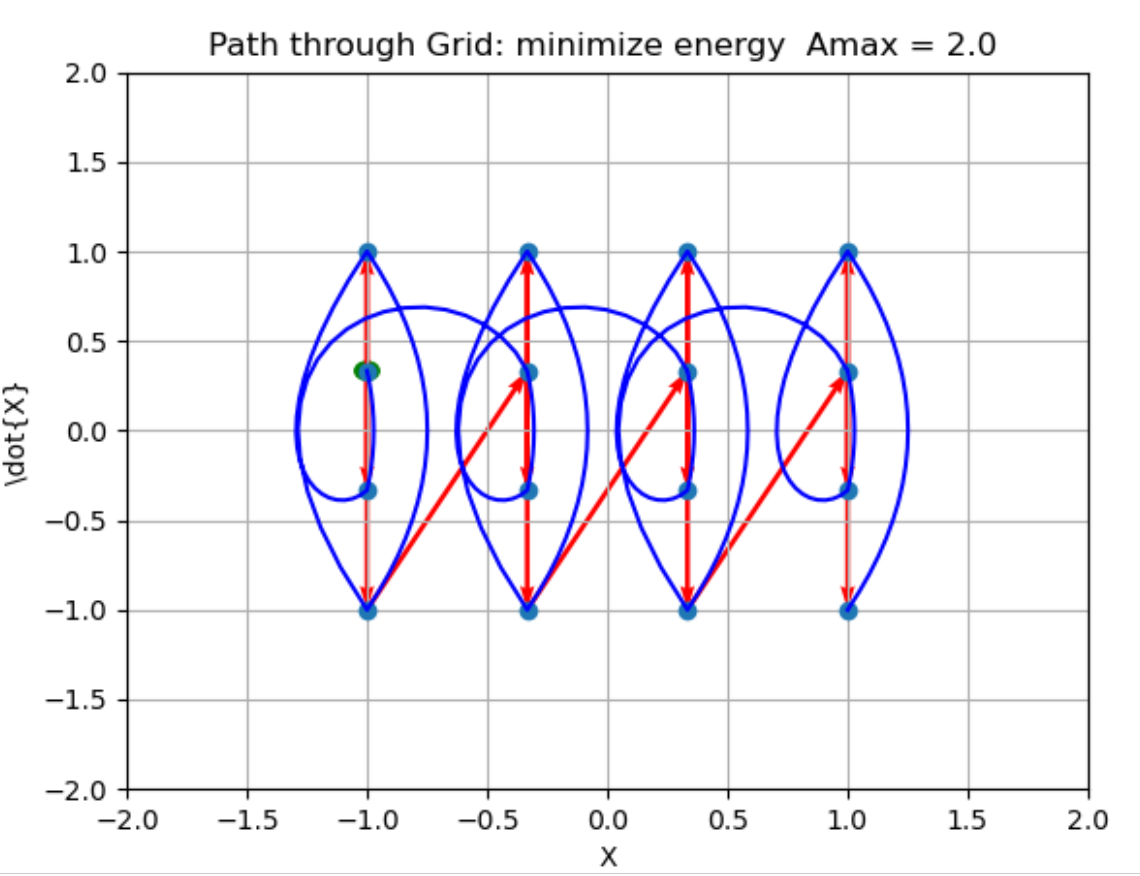
\includegraphics[width=3.0in]{handTraj01.png}
  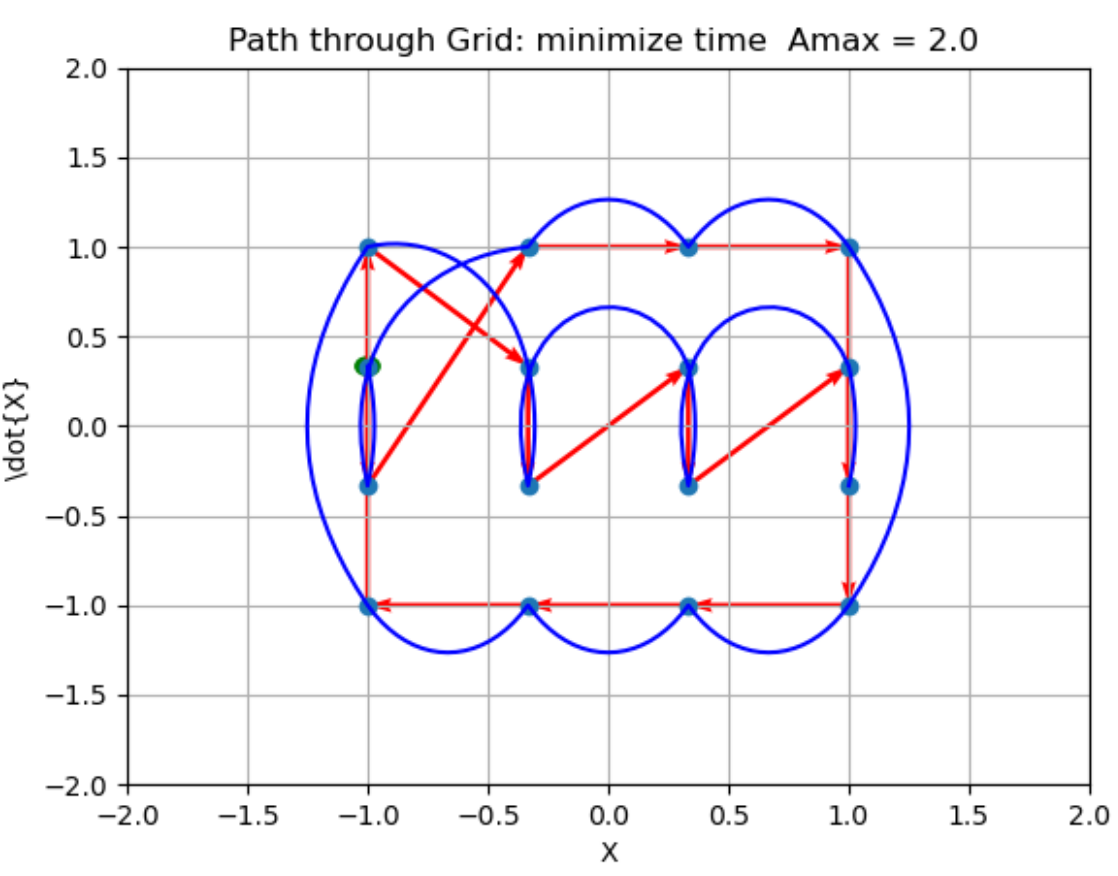
\includegraphics[width=3.0in]{handTraj02.png}
  \caption{}\label{handsolutions1D}
\end{figure}

The two trajectories both start at $X=-1.0$ and $\dot{X}=0.33$
(larger green dot).  The first path minimizes energy cost
and the second minimizes total time.  Both are subject to the
acceleration constraint.

\subsection{simulation structure}
We define the following classes:
\begin{itemize}
  \item {\tt grid}   The grid and associated methods.
  \item {\tt point}  A single point and associated methods.
  \item {\tt trajectory} A trajectory between two points and methods for time-evolution, cost computation.
\end{itemize}

\subsection{overall strategy}

\begin{enumerate}
  \item Create the grid and associated points
  \item Compute for each point, compute the cost of a trajectory between it and all the other points.  Populate
  a cost matrix with $N^6$ rows and $N^6$ columns where
  \beq
    Cm_{ij} = C_x(T_{ij})  \qquad    x \in \{e,t\}
  \eeq
  \item Manually select starting point ($P_0$)
  \item Select the lowest cost column from the starting point row of $Cm$.
  \item Block that point (marking a list)
  \item Repeat until all points are blocked.
\end{enumerate}

\end{document}

